\begin{task}[
  title=Nuclear Medicine application,
  id=opendose-analysis,
  lead=INSERM,
  PM=25,
  wphases={3-33},
  partners={EGI,XFEL}
]

  \textbf{Context}

  % Scientific description
  Nuclear Medicine is a field of medicine where radioactive material
  (radiopharmaceutical) is used for diagnostic and therapy. Even though the
  majority of Nuclear Medicine procedures (90\% according to successive EANM
  surveys) are diagnostic examinations, therapeutic applications tend to
  develop and drag more and more attention, for example for the treatment of
  neuroendocrine tumours \cite{Bodei2009}.

  The formalism used to objectively characterise the irradiation process is
  similar for both application types: it was introduced in the late 60s by the
  MIRD (Medical Internal Radiation Dose) committee of the American Society of
  Nuclear Medicine (SNM). This formalism \cite{loevinger1991mird} requires two
  independent quantities; the radioisotope cumulated activity ($Bq.s$) in the
  source (tissue/organ) and the mean absorbed dose to a given target
  (tissue/organ) per radioisotope disintegration (S-value,
  $Gy.Bq^{-1}.s^{-1}$). The S-value calculation requires a clear definition of
  the geometry of the patient (or the model) and radioisotope decay
  characteristics, it can be expressed as a linear combination of
  yields/energies ($J$) and Specific Absorbed Fractions (SAF, $g^{-1}$).

  The calculation of SAFs involves radiation transport modelling and energy
  deposition scoring in anthropomorphic models, usually based on Monte Carlo
  simulation. Historically, SAFs were computed from mathematical models -
  simplistic approximations to human geometry. The advent of voxel-based
  computational models requires a new appraisal of dosimetric data. For
  example, the models recently proposed by the International Commission on
  Radiation Protection (ICRP) include 140 possible radiation sources, leading
  to around 20000 source/target combinations \cite{ICRP2009ICRPPhantoms}. The
  production of SAFs for these models for all possible source regions,
  radiation types and energiesimpul represent an important computation time
  (millions of CPU hours).

  The OpenDose project \cite{Chauvin2017} is a collaborative effort to generate
  reference dosimetric data using various Monte Carlo codes across different
  teams. The collaboration includes at the moment 14 research teams over 18
  institutes.  The idea is to trigger the collaborative development of a
  reference database, freely available, proposing dosimetric data applicable in
  a context of nuclear medicine dosimetry (for therapy and diagnostic
  applications). A major aspect of the project is the development of tools
  ensuring traceability and reproducibility of generated results.

  % Technical description
  OpenDose data is produced using the five most represented Monte Carlo
  simulation software in medical applications: Geant4/GATE, MCNP, EGS, PENELOPE
  and Fluka. Each simulation consists of calculating radiation transport in
  anthropomorphic models for specific parameters (source organ, particle type,
  energy, model and number of primaries to simulate). Every simulation produces
  binary (3D matrices) and ASCII files for a total of $\sim$150MB / simulation.
  The 3D matrices contain energy deposited per voxels, and ASCII files contain
  pre-processed data corresponding to energy deposited per regions such as
  organs and tissues. These raw outputs are later processed into dosimetric
  data such as Specific Absorbed Fractions (SAFs) and S-values.

  Producing data for one model (ex. adult female) requires $\sim$30,000
  simulations, with the workload shared between the different teams and
  software.

  The data produced by all the teams is currently centralised at the Cancer
  Research Center of Toulouse (CRCT), processed and fed into a local SQL
  database at CRCT.

  This collaborative effort raises some challenges:
  \begin{compactitem}
  \item Data production: a total of 750,000 hours of CPU time is needed per
    model.
  \item Volume of data: one model represents TB of raw data that can be
    heterogeneous from the different teams.
  \item Data analysis: raw data has to be processed into dosimetric data in a
    robust and reproducible way.
  \item Database: has to be efficient and handle all the data (raw and
    processed).
  \item Visualization: display and compare results from all teams.
  \end{compactitem}

  \textbf{This task}

  The objective of this task is to build on the Jupyter ecosystem to create a
  unified data analysis framework for the OpenDose project. Figure
  \ref{fig:opendose_framework} shows the overall framework of the project and
  how data will be managed.

  \begin{figure}[t!]
    \centering
    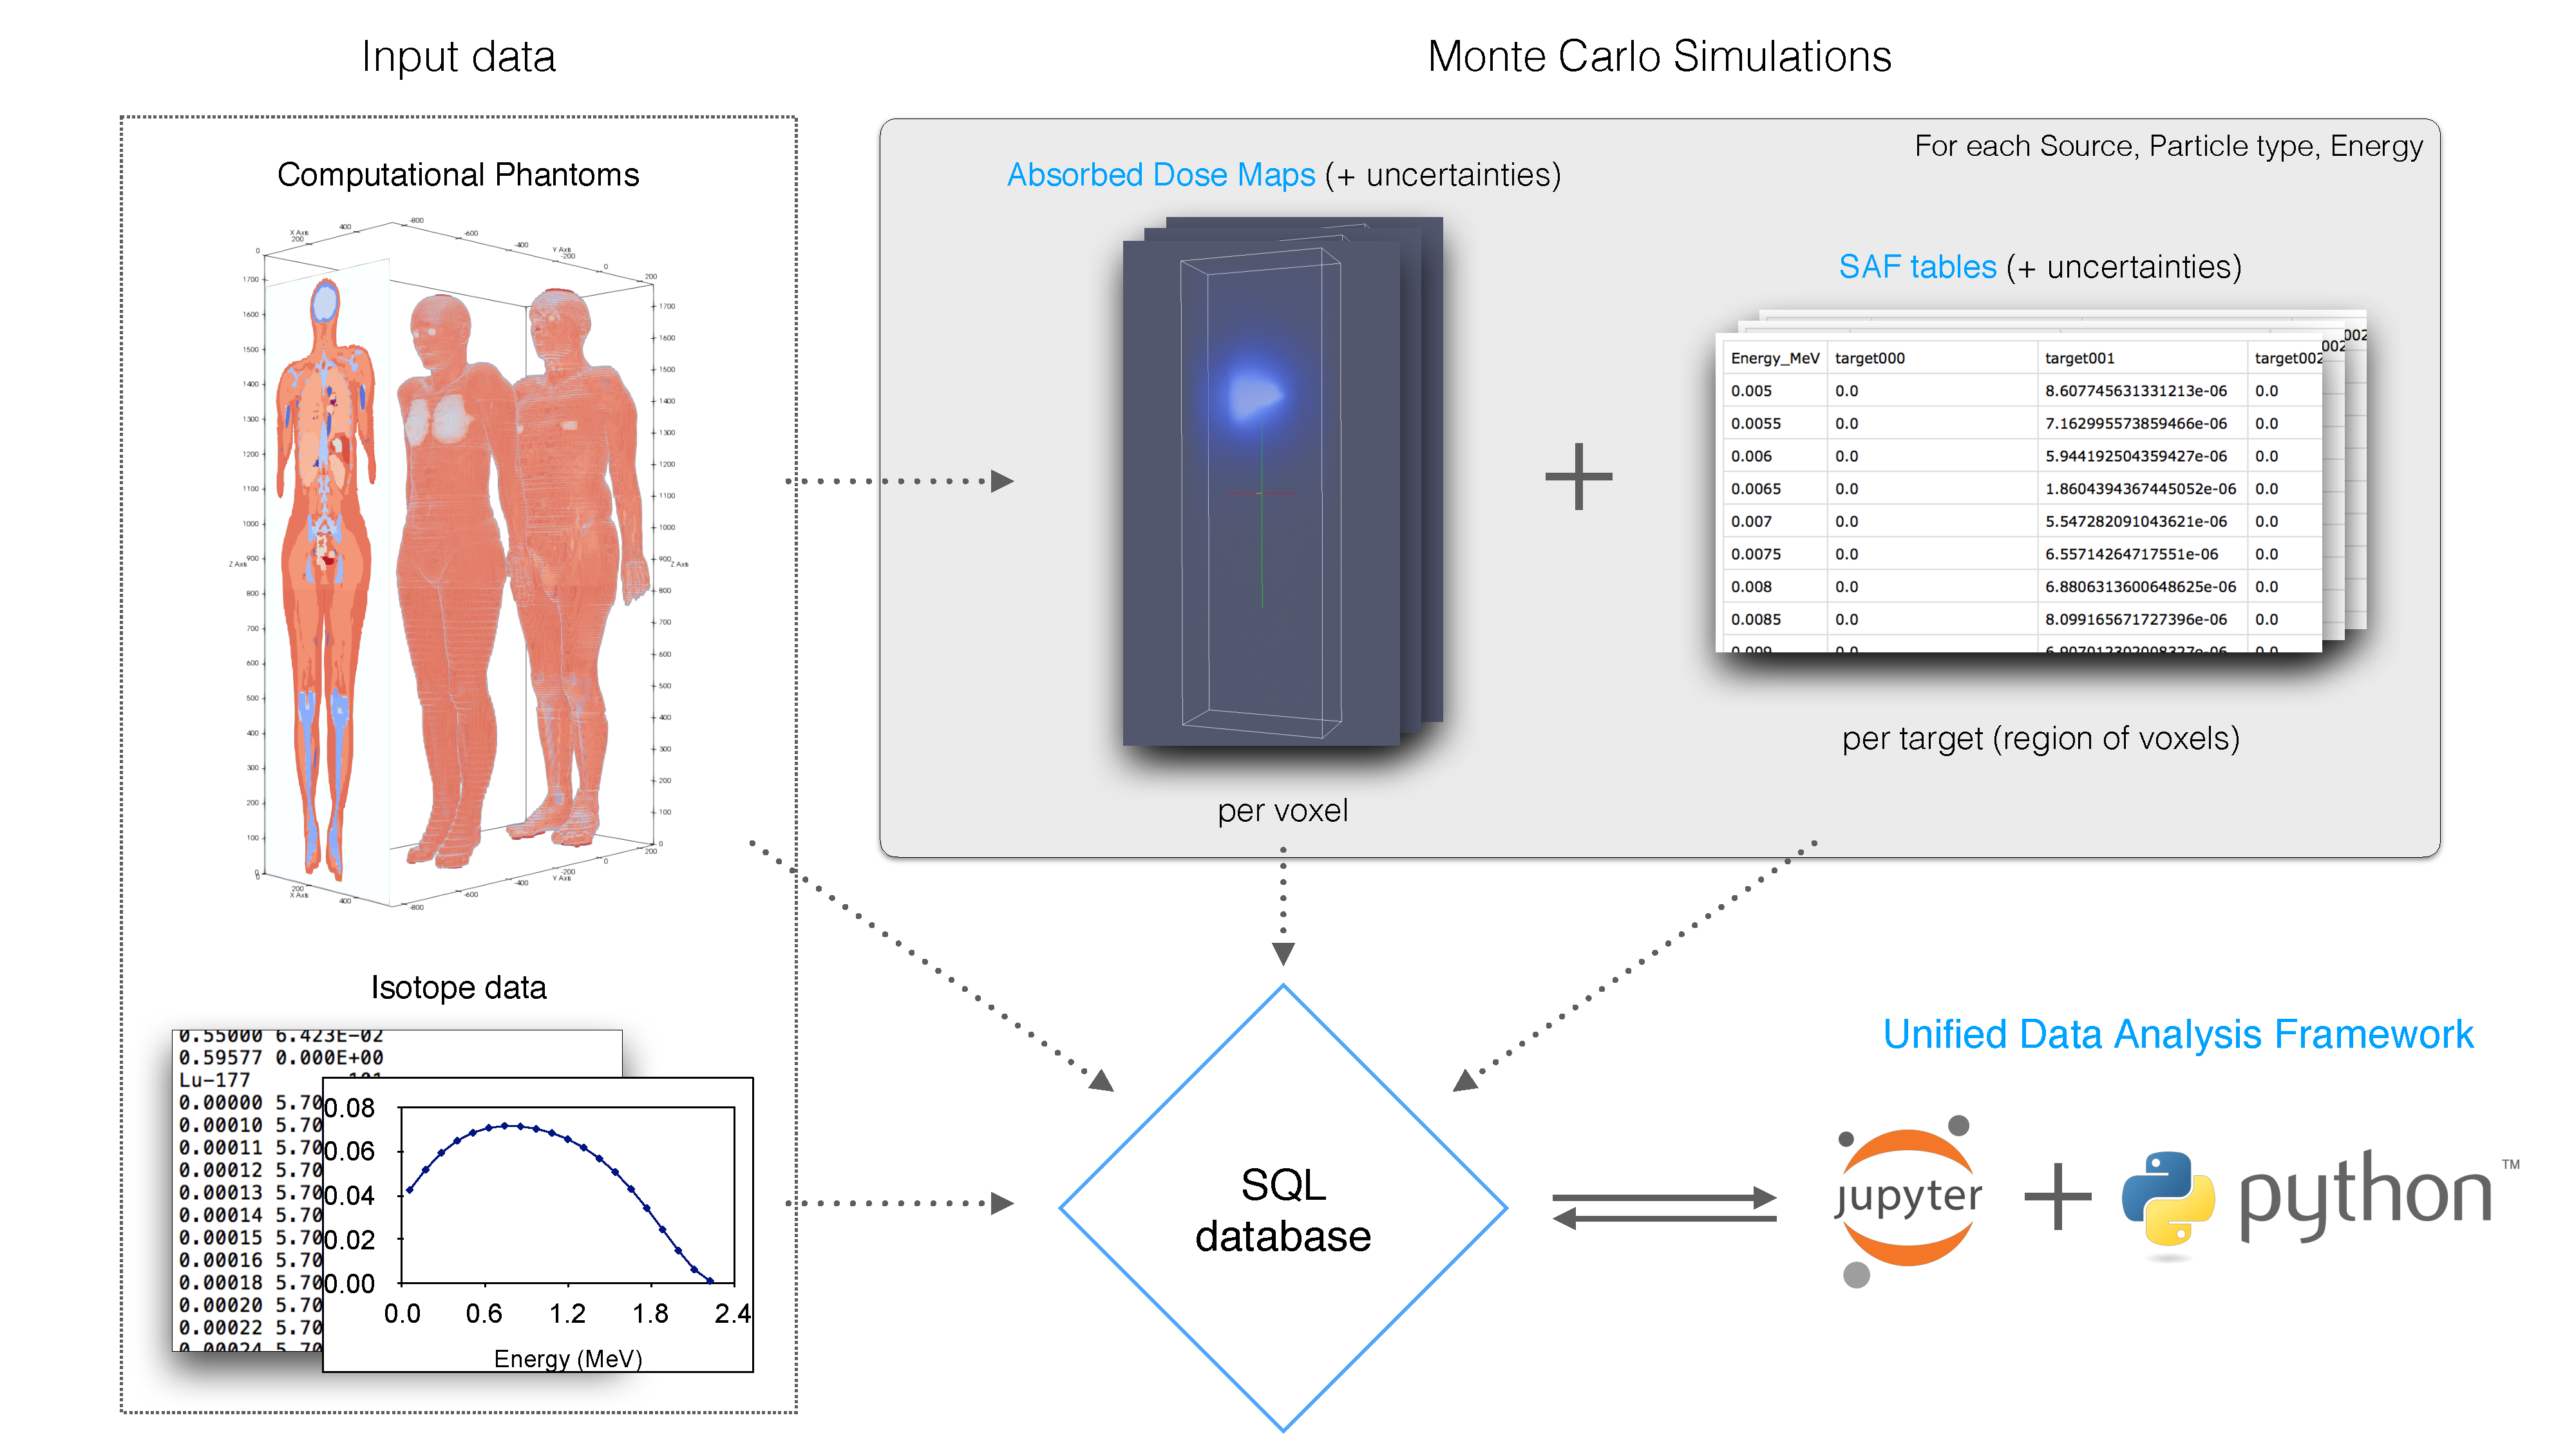
\includegraphics[width=1.0\textwidth]{images/opendose_framework.pdf}
    \caption{OpenDose project overall framework including the unified data
    analysis to be developed in this task.}
    \label{fig:opendose_framework}
  \end{figure}
  
  By building a set of tools to access and process data, this will ensure the
  production of traceable and reproducible dosimetric data for the OpenDose
  project members.

  Another major aspect of the OpenDose collaboration is to provide an open
  access to the generated dosimetric data. For that purpose a website is under
  development to allow data download and simple dosimetry calculations. For
  users who need more advanced calculations, a dedicated Jupyter workspace will
  provide a set of tools to easily access, process and display the OpenDose
  data.

  The task includes the following activities:
  \begin{compactitem}
  \item Developing tools to work seamlessly on the SQL database holding the
    dosimetric data.
  \item Developing data analysis tools using the Python data science ecosystem
    where possible.
  \item Developing visualization tools, exploring Widgets inside the Notebook
    for interactivity.
  \item Evaluate the relevance of Jupyter Notebooks from user feedback
  \item Disseminating results.
  \item Providing support to users.
  \end{compactitem}
  First, these developments will be available to users as Jupyter Notebooks to
  be run locally on their machines. In a second time, these Notebooks will be
  ported on the European Binder instance following developments of task
  \taskref{eosc}{eu-binder}. The reproducibility of generated results will be
  ensured by archiving the software environment with developments of task
  \taskref{ecosystem}{reproducibility}.

  The deliverable of this task will be a demonstrator
  (\localdelivref{opendose-analysis}) available via the EOSC hub, contributing
  to the development of innovatives services for the scientific community.

  The evaluation of the developed tools from user feedback will contribute to
  the deliverable \localdelivref{applications-report}.

  \TODO{How does this task relate to EOSC-life?}

\end{task}
